% $Header$

\documentclass{beamer}

% This file is a solution template for:

% - Talk at a conference/colloquium.
% - Talk length is about 20min.
% - Style is ornate.



% Copyright 2004 by Till Tantau <tantau@users.sourceforge.net>.
%
% In principle, this file can be redistributed and/or modified under
% the terms of the GNU Public License, version 2.
%
% However, this file is supposed to be a template to be modified
% for your own needs. For this reason, if you use this file as a
% template and not specifically distribute it as part of a another
% package/program, I grant the extra permission to freely copy and
% modify this file as you see fit and even to delete this copyright
% notice. 


\mode<presentation>
{
  %\usetheme{Berkeley}
  %\usetheme{Warsaw}
  \usetheme{CambridgeUS}
  % or ...

  \setbeamercovered{transparent}
  % or whatever (possibly just delete it)
}


\usepackage[english]{babel}
% or whatever

\usepackage[utf8]{inputenc}
% or whatever

\usepackage{times}
%\usepackage[T1]{fontenc}
% Or whatever. Note that the encoding and the font should match. If T1
% does not look nice, try deleting the line with the fontenc.

\usepackage[font=footnotesize,labelformat=empty,
            justification=raggedright,
%            singlelinecheck=false
  ]{caption}
  
\usepackage{upgreek}
  
\title[Graph Cut - Final Presentation] % (optional, use only with long paper titles)
{Graph Cut}

\subtitle
{Final Presentation}

\author[Bruno C. Fiss, Max Göttner] % (optional, use only with lots of authors)
{Bruno Coswig Fiss \and Max Göttner}
% - Give the names in the same order as the appear in the paper.
% - Use the \inst{?} command only if the authors have different
%   affiliation.

\institute[TU Berlin] % (optional, but mostly needed)
{
  \inst{1}%
  Institut für Technische Informatik und Mikroelektronik\\
  Technische Universität Berlin}
% - Use the \inst command only if there are several affiliations.
% - Keep it simple, no one is interested in your street address.

\date[\today] % (optional, should be abbreviation of conference name)
{Parallele Algorithmen auf GPUs}
% - Either use conference name or its abbreviation.
% - Not really informative to the audience, more for people (including
%   yourself) who are reading the slides online

\subject{Image processing}
% This is only inserted into the PDF information catalog. Can be left
% out. 



% If you have a file called "university-logo-filename.xxx", where xxx
% is a graphic format that can be processed by latex or pdflatex,
% resp., then you can add a logo as follows:
% graphics stuff

%\usepackage{pgf}
\pgfdeclareimage[interpolate=true,height=1.0cm]{university-logo}{TUBerlin_Logo_rot}
\logo{\pgfuseimage{university-logo}}

\pgfdeclareimage[interpolate=true,height=5.0cm]{formula}{formula}

% (6) the launch timed out and was terminated

% Delete this, if you do not want the table of contents to pop up at
% the beginning of each subsection:
\AtBeginSection[]
{
  \begin{frame}<beamer>{Outline}
    \tableofcontents[currentsection]
  \end{frame}
}


% If you wish to uncover everything in a step-wise fashion, uncomment
% the following command: 

%\beamerdefaultoverlayspecification{<+->}


\begin{document}

\begin{frame}
  \titlepage
\end{frame}

\begin{frame}{Outline}
  \tableofcontents
  % You might wish to add the option [pausesections]
\end{frame}


% Structuring a talk is a difficult task and the following structure
% may not be suitable. Here are some rules that apply for this
% solution: 

% - Exactly two or three sections (other than the summary).
% - At *most* three subsections per section.
% - Talk about 30s to 2min per frame. So there should be between about
%   15 and 30 frames, all told.

% - A conference audience is likely to know very little of what you
%   are going to talk about. So *simplify*!
% - In a 20min talk, getting the main ideas across is hard
%   enough. Leave out details, even if it means being less precise than
%   you think necessary.
% - If you omit details that are vital to the proof/implementation,
%   just say so once. Everybody will be happy with that.

\section{Introduction}
\subsection{Short Description of the Problem}

\begin{frame}{Using Graph Cut for Energy Minimization}
  % - A title should summarize the slide in an understandable fashion
  %   for anyone how does not follow everything on the slide itself.
   Minimize:
   \begin{figure}
   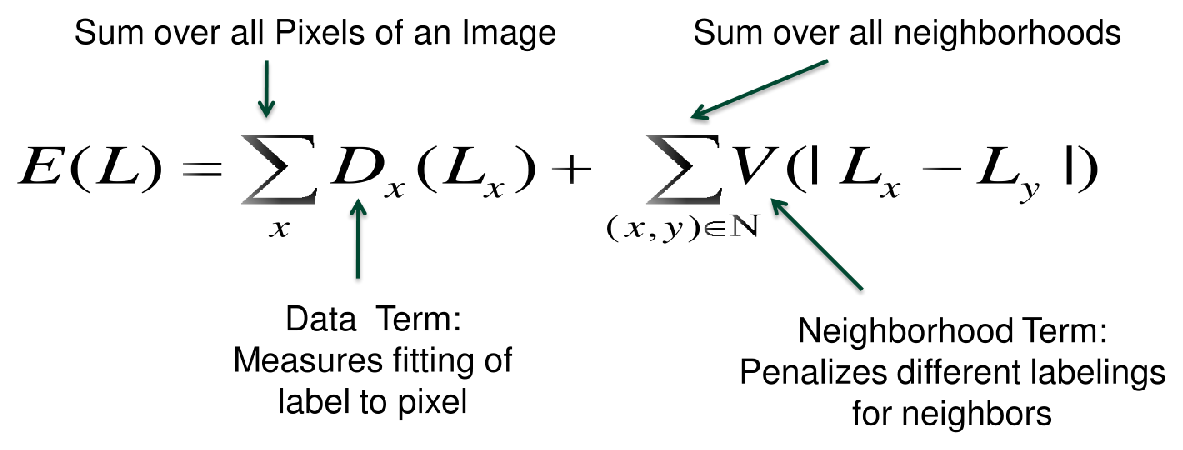
\includegraphics[scale=0.5]{formula} 
   \captionof{figure}{\scriptsize Credit:\thinspace{\small\itshape Timo Stich, 2009}}
   \end{figure}
\end{frame}

\begin{frame}{Using Graph Cut for Energy Minimization}
  % - A title should summarize the slide in an understandable fashion
  %   for anyone how does not follow everything on the slide itself.
   Find minimum cut:
   \begin{figure}
   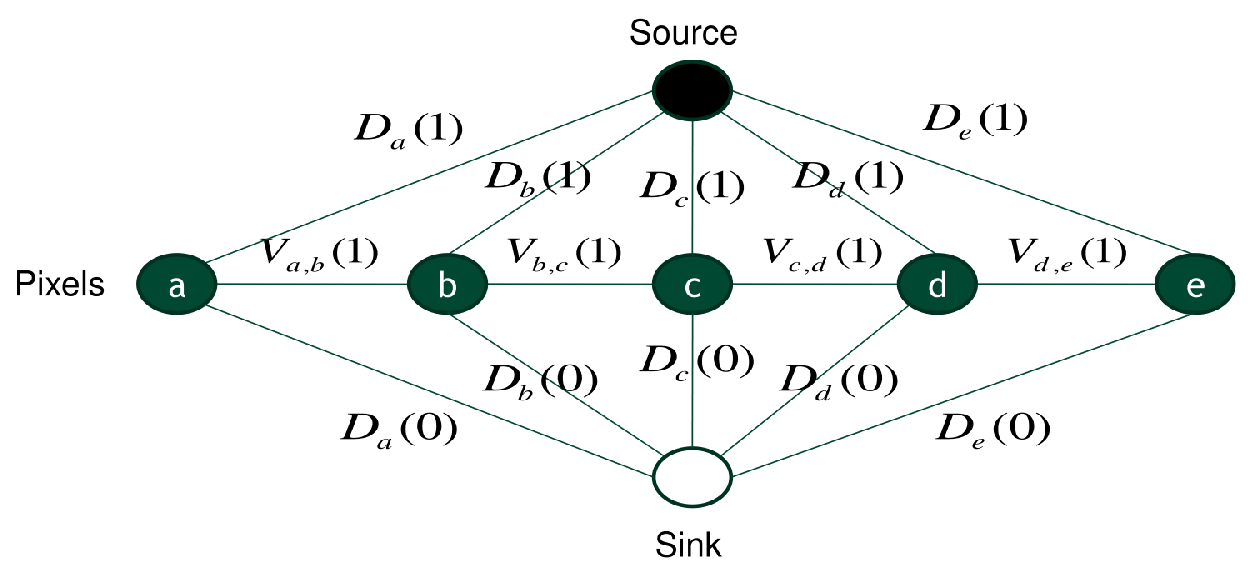
\includegraphics[scale=0.5]{graph} 
   \captionof{figure}{\scriptsize Credit:\thinspace{\small\itshape Timo Stich, 2009}}
   \end{figure}
\end{frame}

\begin{frame}{Using Graph Cut for Energy Minimization}
  % - A title should summarize the slide in an understandable fashion
  %   for anyone how does not follow everything on the slide itself.
   Find minimum cut:
   \begin{figure}
   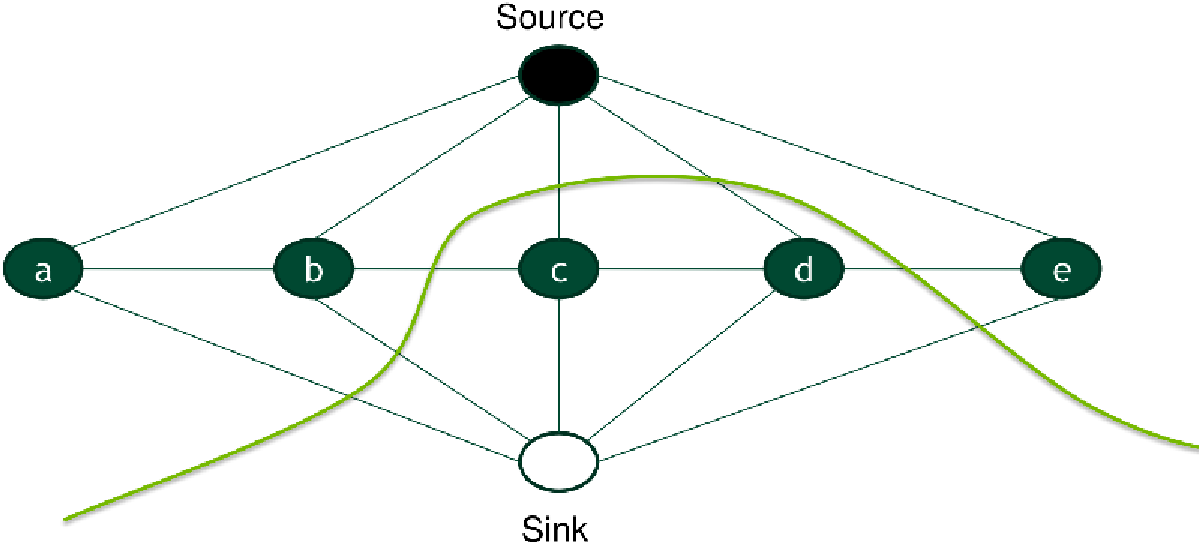
\includegraphics[scale=0.5]{graph2} 
   \captionof{figure}{\scriptsize Credit:\thinspace{\small\itshape Timo Stich, 2009}}
   \end{figure}
\end{frame}

\subsection{Parallelization Opportunities}

\begin{frame}{Flow is moving...}
	  \begin{itemize}
	    \item
	    Major oportunity: Make more than one flow move in parallel.
	  \end{itemize}
\end{frame}

\section{Solution}

\subsection{Main Ideas}

\begin{frame}{Conflicts}
\begin{itemize}
 \item
 Every thread is responsible for one node/pixel.
 \item
 Apply Push and Relabel to every node.
 \item
 \alert{How to avoid conflicts?}
\end{itemize}
\end{frame}

\begin{frame}{Conflicts}
\begin{itemize}
 \item
 Every thread is responsible for one node/pixel.
 \item
 Apply Push and Relabel to every node.
 \item
 \alert{How to avoid conflicts?}
 \item
 Dividing kernel in parts or using atomic operations.
\end{itemize}
\end{frame}

\begin{frame}{Convergence}
\begin{itemize}
 \item
 Every thread is responsible for one node/pixel.
 \item
 Apply Push and Relabel to every node. \alert{Repeat it until flow stops changing.}
\end{itemize}
\end{frame}

\begin{frame}{Convergence}
\begin{itemize}
 \item
 Every thread is responsible for one node/pixel.
 \item
 Apply Push and Relabel to every node. \alert{Repeat it until flow stops changing?}
 \item
 Convergence is too slow $\rightarrow$ Global Relabel.
\end{itemize}
\end{frame}

\subsection{Speeding Up}

\begin{frame}{Global Relabel}
\begin{itemize}
 \item
 Global Relabel: Read \alert{every} neighbor edge, get label if connected.
 \item
 Compress neighborhood!
\end{itemize}
\end{frame}

\begin{frame}{Global Relabel}
\begin{itemize}
 \item
 Global Relabel: After changing label, inactive.
 \item
  \_\_syncthreads\_or(comp\_n \& (1 $<<$ 8))
\end{itemize}
\end{frame}

\begin{frame}{Push}
\begin{itemize}
 \item
 Push: Reads every neighbor's height.
 \item
 Shared memory!
 \item
 or compress!
\end{itemize}
\end{frame}

\begin{frame}{Push}
\begin{itemize}
 \item
 Push: Excess is written by the owner thread and by neighbors.
 \item
 Shared memory?
 \item
 Not good. Perhaps too many \_\_syncthreads().
 \item
 Better stay with atomic? Or Timo Stich's Wave...
\end{itemize}
\end{frame}

\begin{frame}{Extra}
\begin{itemize}
 \item
 Suitable block size (32x8 and 88-100\%).
 \item
 Block activity list.
\end{itemize}
\end{frame}

\section{Results}

\subsection{Performance Comparison}

\begin{frame}{Comparison with Previous Works}
\begin{itemize}
\item
CudaCuts by Vibhav Vineet and P. J. Narayanan, 2008.
\item
Fastest known CPU implementation by Boykov \emph{et al.}.
\item
Fastest known GPU implementation (current NPP implementation [Timo Stich 2011])
\item
On the same dataset (changing size) = proportion is constant, 2-3x slower than NPP.
\end{itemize}

 \begin{tabular}{|c|c|c|c|c|}
\hline
\textbf{Dataset}   &  \textbf{CPU}    & \textbf{CudaCuts} & \textbf{Ours}    & \textbf{NPP} \\
\hline
Flower (600x450)   &  191 ms & 18 ms    & 9 ms    & 5 ms   \\
Sponge (640x480)   &  268 ms & 21 ms    & 10 ms   & 4 ms   \\
Person (600x450)   &  210 ms & 28 ms    & 13 ms   & 9 ms   \\
Rihanna (3600x3600)&  N/A    & 748 ms   & 450 ms  & 150 ms \\
\hline
\end{tabular}
\end{frame}


\subsection{Application}


\section{Conclusions}

\begin{frame}{Final Remarks}
\begin{itemize}
 \item
 Performance beats reasonably recent implementations.
 \item
 Many things tried out.
 \item
 Still lots to learn.
\end{itemize}
\end{frame}

\section*{Thank you!}

\begin{frame}{Conclusion}

  % Keep the summary *very short*.
  \begin{itemize}
  \item
    \alert{Thank you!}
  \end{itemize}
  
  % The following outlook is optional.
  \vskip0pt plus.5fill
  \begin{itemize}
  \item
    Some additional material and references:
    \begin{itemize}
    \item
      \url{http://cvit.iiit.ac.in/papers/rtGCuts_2008.pdf}
    \item
      \url{http://www.nvidia.com/content/GTC/documents/1060_GTC09.pdf}
    \item
      \url{http://vision.middlebury.edu/}
    \end{itemize}
  \end{itemize}
\end{frame}


\end{document}


